% 独自のコマンド

% ■ アブストラクト
%  \begin{jabstract} 〜 \end{jabstract}  :日本語のアブストラクト
%  \begin{eabstract} 〜 \end{eabstract}  :英語のアブストラクト

% ■ 謝辞
%  \begin{acknowledgment} 〜 \end{acknowledgment}

% ■ 文献リスト
%  \begin{bib}[100] 〜 \end{bib}


\newif\ifjapanese

\japanesetrue  % 論文全体を日本語で書く(英語で書くならコメントアウト)

\ifjapanese
  \documentclass[a4j,twoside,openright,11pt]{jreport} % 両面印刷の場合。余白を綴じ側に作って右起こし。
  %\documentclass[a4j,11pt]{jreport}                  % 片面印刷の場合。
  \renewcommand{\bibname}{参考文献}
  \newcommand{\acknowledgmentname}{謝辞}
\else
  \documentclass[a4paper,11pt]{report}
  \newcommand{\acknowledgmentname}{Acknowledgment}
\fi
\usepackage{thesis}
\usepackage{ascmac}
\usepackage[dvipdfmx]{graphicx}
\usepackage{multirow}
\usepackage{url}
\bibliographystyle{jplain}

\bindermode  % バインダー用余白設定

% 日本語情報(必要なら)
\jclass  {修士論文}                             % 論文種別
\jtitle    {ユーザのコンテキストを利用したテキスト入力システムの研究}    % タイトル。改行する場合は\\を入れる
\juniv    {慶應義塾大学大学院}                  % 大学名
\jfaculty  {政策・メディア研究科}               % 学部、学科
\jauthor  {臼杵 壮也}                       % 著者
\jhyear  {26}                                   % 平成○年度
\jsyear  {2014}                                 % 西暦○年度
\jkeyword  {IME、日本語入力、コンテキスト、推薦}     % 論文のキーワード
\jproject{インタラクションデザインプロジェクト} %プロジェクト名
\jdate{2015年1月}

% 英語情報(必要なら)
\eclass  {Master's Thesis}                            % 論文種別
\etitle    {Development of a context-based text input system}      % タイトル。改行する場合は\\を入れる
\euniv  {Keio University}                             % 大学名
\efaculty  {Graduate School of Media and Governance}  % 学部、学科
\eauthor  {Usuki Masaya}                           % 著者
\eyear  {2014}                                        % 西暦○年度
\ekeyword  {Input Method Editor,
            Japanese, Context, recommend}          % 論文のキーワード
\eproject{Interaction Design Project}                 %プロジェクト名
\edate{January 2015}





\begin{document}

\ifjapanese
  \jmaketitle    % 表紙(日本語)
\else
  \emaketitle    % 表紙(英語)
\fi

% ■ アブストラクトの出力 ■
%	◆書式:
%		begin{jabstract}〜end{jabstract}	:日本語のアブストラクト
%		begin{eabstract}〜end{eabstract}	:英語のアブストラクト
%		※ 不要ならばコマンドごと消せば出力されない。



% 日本語のアブストラクト
\begin{jabstract}

モバイルデバイスの進化と普及と共に文字入力の機会は増加している。
しかし現状スマートフォンを利用してる人々の
日本語入力IMEには大きな変化はみられない。
本研究では現状のモバイルデバイスに適した、
より早く面白い入力を可能にする日本語入力IME
「Rive日本語入力」を設計し実装した。
本システムにおける最大の特徴はコンテキストを用いた
候補単語の推薦を行うことである。
コンテキストと入力を関連付けると共に、
過去の全てのユーザーの入力データを利用することで
ユーザーの入力したいであろう単語を推測する。
ユーザーは意識することなく推薦候補単語を受け取り、
選択するだけで入力をすることができる。
本論文においては
開発した日本語入力IMEの設計や実装、
採用したユーザインタフェースを提示することで、
システムの有用性を述べる。
また本システムの課題やそれに対するアプローチを述べることで、
日本語入力IMEにおける本研究の意義を論ずる。

\end{jabstract}

% 英語のアブストラクト
\begin{eabstract}

We are increasing at an opportunity to input text
with evolution and the spread of mobile devices.
But smartphone user's inputting hardly changes in Japanese IME.
In this research, I designed and implemented Japanese IME:
"Rive Japanese Input" which enables the quick input
and interesting input of the user.
The biggest feature of this system is to recommend candidate words
from the context.
I connect input data with context and suppose the text
that the user want to input by using the past input data
of all users
The user receives recommendation candidate words unconsciously.
And he complete input only to choose words in recommendation
candidate words.
In this paper, I propose usability of this system by adopting
user interface and the implementation of Japanese IME which
I developed.
And I discuss importance of this study.

\end{eabstract}
  % アブストラクト。要独自コマンド、include先参照のこと

\tableofcontents  % 目次
\listoffigures    % 表目次
\listoftables    % 図目次

\pagenumbering{arabic}

\chapter{序論}
\label{chap:introduction}
本章では研究の目的、使用する用語の定義と
論文の構成について述べる。

\newpage
\section{研究の目的}
本研究の目的は世の中の日本語を入力する人々が
コンピュータあるいはモバイルデバイスへの入力を行う際に、
ユーザの文字入力における楽しさを向上させると共に
文字入力の速度を向上させることが目的である。
その目的を達成するためにRive日本語入力というシステムを実装・開発した。

\section{用語定義}
本論文において使用する用語を以下のように定義する。

\begin{description}
  \item[デバイス]\mbox{}\\
    本論文に置いてデバイスとは単にハードウェアを意味している。
  \item[モバイルデバイス]\mbox{}\\
    本論文において、モバイルデバイスとは持ち運び可能であり、
    インターネットに接続可能な端末のことを意味している。
  \item[スマートフォン]\mbox{}\\
    本論文において、スマートフォンとは多機能なモバイルデバイスであり、
    パソコンとしての機能を果たせるものを意味している。
    具体的にはAndroid,iOSなどを搭載しているものである。
  \item[タブレット]\mbox{}\\
    本論文において、スマートフォンと同じ要件を満たしながら、
    画面のサイズがスマートフォンより大きい物を意味している。
  \item[IME]\mbox{}\\
    IMEとはInput Method Editorの略であり
    文字入力補助ソフトと言われる。。
    コンピュータなどの情報機器において文字入力をする際に、
    それを手助けするシステムのことをIMEと呼ぶ。
  \item[コンテキスト]\mbox{}\\
    コンテキストとは本論文において状況という意味で使っている。
  \item[集合知]\mbox{}\\
    集合知とは複数のデータを集める事によって
    新たな価値を出すという意味で使っている。
  \item[省入力]\mbox{}\\
    本論文において省入力とは
    入力の時間または手間を省くことを示している。
  \item[候補単語]\mbox{}\\
    本論文に置いて候補単語とは入力における、
    変換候補と推薦候補の二つを合わせた表現である。
  \item[クライアント]\mbox{}\\
    本論文においてクライアントとは
    ユーザーが直接利用するアプリケーション
    あるいはそのデバイスを指す表現である。
\end{description}

\section{本論文の構成}
第\ref{chap:background}章ではRive日本語入力の開発に至った背景について述べる。
第\ref{chap:design}章ではRive日本語入力の設計について述べる。
第\ref{chap:recommend}章では推薦システムの使用について述べる。
第\ref{chap:implementation}章ではRive日本語入力の実装について述べる。
第\ref{chap:userinterface}章ではRive日本語入力のユーザーインターフェースについて述べる。
第\ref{chap:discussion}章ではRive日本語入力の課題について述べる。
第\ref{chap:related}章では関連研究を述べる。
第\ref{chap:conclusion}章では本研究の結論を述べる。
最後に第\ref{chap:publication}章では研究に関する発表について述べる。

\chapter{背景}
\label{chap:background}
本章では本研究の背景となった、
モバイルデバイスへの文字入力機会増加、入力のシステム歴史、文字入力への問題
について述べる。

\newpage
\section{モバイルデバイスへの文字入力の機会の増加}
モバイルデバイスにおいて、文字入力をする機会がとても多い。

\subsection{モバイルデバイスの普及}
現在、日本において
スマートフォンやタブレットなどのモバイルデバイスが大幅かつ急激に普及した。
総務省による「平成25年通信利用動向調査」
\cite{communicationreport}の
「通信端末世帯保有率の推移」
(図:\ref{fig:mobiledevicespread})によると、
\begin{figure}[htbp]
  \begin{center}
    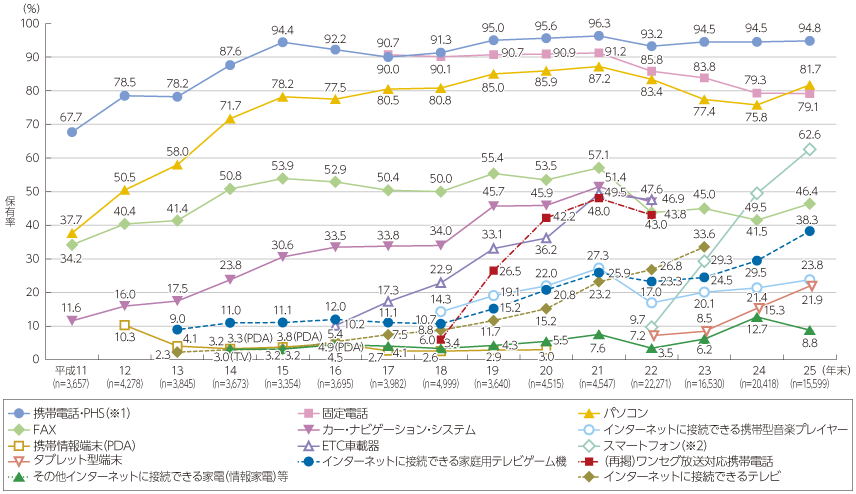
\includegraphics[width=160mm,bb=0 0 856 494]{images/mobiledevicespread.png}
    \caption{情報通信端末世帯保有率の推移(出典:\cite{communicationreport})}
    \label{fig:mobiledevicespread}
  \end{center}
\end{figure}
平成22年には9.7%しかなかったスマートフォンの普及率は、
平成25年には62.6%と急激に成長している。
平成22年から平成25年の3年間で52.9%の伸びを見せており、
これはパソコンの保有率が最も伸びた平成11年から平成14年の
伸び率を大きく上回る数字となっている。
このデータからもスマートフォンの普及は未だかつてないほどの
速度で進んでいることがわかる。

\subsection{モバイルデバイスの用途}
スマートフォンはパソコンの様に多くのことができるが、
文字入力を行う可能性が高いアプリケーションは頻繁に使用されている。
リサーチバンクによるアンケート調査\cite{researchbanksmartphone}
(図:\ref{fig:purpose})によると
\begin{figure}[htbp]
  \begin{center}
    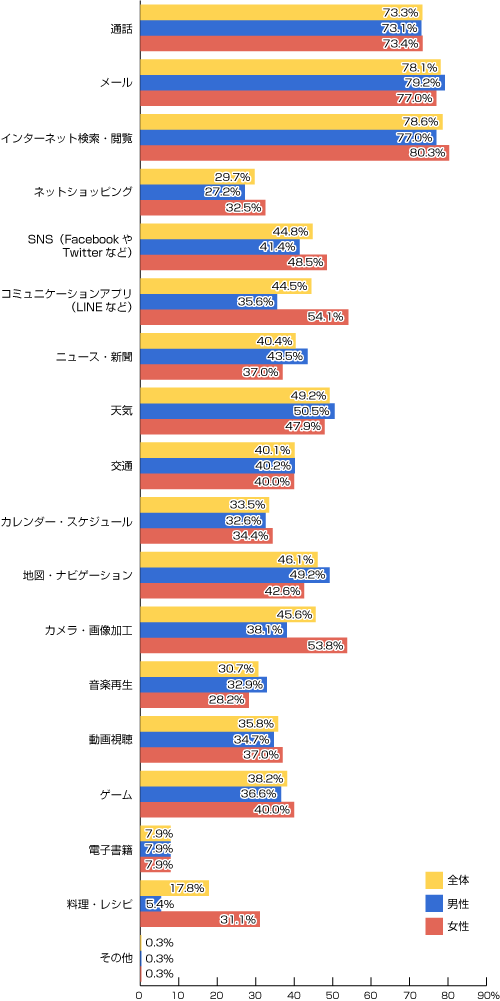
\includegraphics[width=115mm,bb=0 0 500 1001]{images/purpose.png}
    \caption{スマートフォンでどのような機能・アプリを使っているか(出典:\cite{researchbanksmartphone})}
    \label{fig:purpose}
  \end{center}
\end{figure}
メールアプリを使う人が78.1%、SNSアプリを使う人が44.8%、
コミュニケーションアプリを使う人が44.5%となっている。
メールアプリ、コミュニケーションアプリ、SNSアプリはそれぞれ
情報の受信端末としてだけ使う場合には文字入力の必要はないが、
情報を発信しようとする場合には文字入力が必要である。
これら以外の他のアプリにおいても適時文字入力が必要である。
つまりスマートフォンを使うユーザーは文字入力の機会がとても多いことがわかる。
またデバイスが多様化し、文字入力の機会が増えている。
スマートウォッチ(図:\ref{fig:smartwatch})や、
HMDの一つであるGoogle Glass(図:\ref{fig:googleglass})がその例である。
\begin{figure}[htbp]
  \begin{minipage}{0.5\hsize}
    \begin{center}
      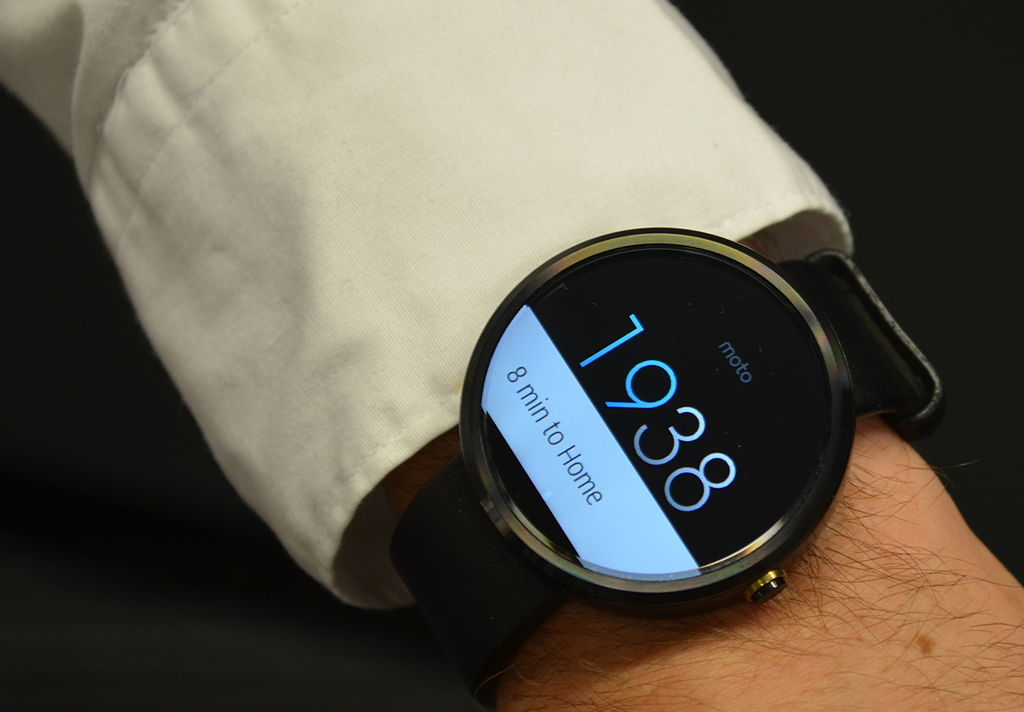
\includegraphics[width=70mm,bb=0 0 246 171]{images/smartwatch.png}
    \end{center}
    \caption{スマートウォッチの例:Android Wearを搭載したMoto360(出典:\cite{smartwatch})}
    \label{fig:smartwatch}
  \end{minipage}
  \begin{minipage}{0.5\hsize}
    \begin{center}
      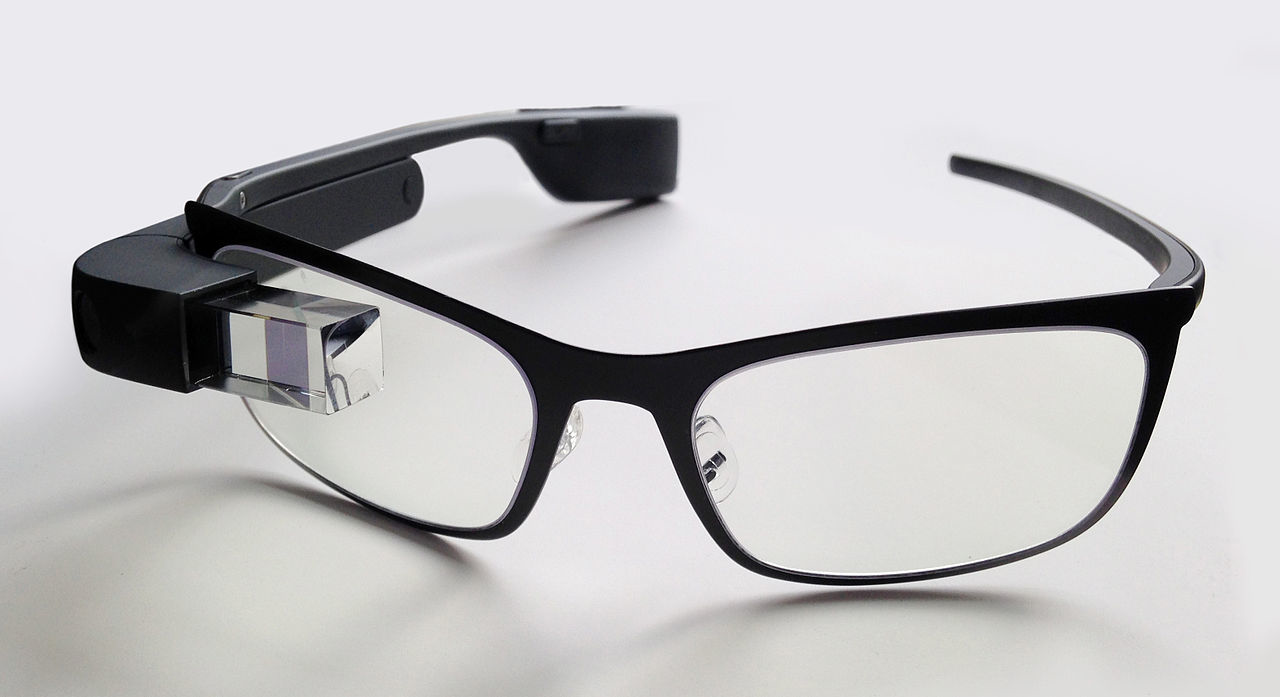
\includegraphics[width=70mm,bb=0 0 1280 697]{images/googleglass.png}
    \end{center}
    \caption{Google glass(出典:\cite{googleglass})}
    \label{fig:googleglass}
  \end{minipage}
\end{figure}
スマートウォッチは既存の時計にモバイルデバイスOSを搭載したもので、
従来の時計であれば文字入力とは無縁であったが、
これを使うことで、文字入力をこのデバイス上でも
行う必要が出てくる。


\section{日本語と英語入力の差異}
日本語と英語では入力にかかるコストが異なる。
qwertyキーボードで日本語を入力する場合、
アルファベットを入力し、それをひらがなに日本語IMEが変換し、
それを漢字やカタカナの混ざった文章に変換するというプロセスをとる。
英語においては入力したアルファベットがそのまま文章となるため、
IMEの必要がなく、ほとんど使われていないのが現状である。

\section{入力システムの変遷}
現在どのようなOSを使用していても必ずIMEアプリケーションは搭載されている。
これらのモバイルデバイスを使う上で日本語の入力は欠かすことができない操作である。
デバイスの性能は携帯電話の頃から劇的に向上している。
パソコンに遜色ないようなメモリやCPUを積んでいるものも多く市販されている。
しかしIMEのシステムに関しては携帯電話の時から大きな変化はない。
日本語IMEにおける内部的なシステムとしては、
連文節変換や予測入力\cite{pobox}の導入がおこなわれ、
広く普及したがまだ改善の余地は多い。
文字入力の方法についても

文字入力にもデバイスに適したよりよいものがある。
文字入力のユーザの体験ももっと向上すべきである。
今回は日本人向けのシステムとして作った。

ユーザにはそれぞれコンテキストがある。
コンテキストによって入力したい単語は推測できるのではないか

\section{問題点と期待}
IMEに関する問題点と期待について述べる。

\subsection{問題点}
楽天リサーチによる「スマートフォンに関する調査」
(出典:\cite{rakutensmartphone})によると、
スマートフォンを使うユーザーが挙げる不満点の中で
最も割合が大きいのが「文字入力がしにくい」ということである。
(出典:\cite{rakutensmartphone})
\begin{figure}[htbp]
  \begin{center}
    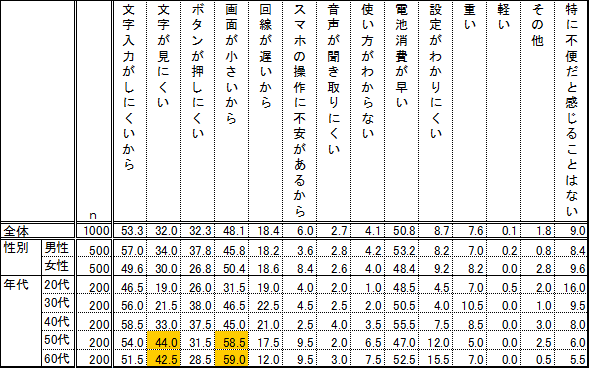
\includegraphics[width=140mm,bb=0 0 589 368]{images/dissatisfaction.png}
    \caption{スマートフォンを利用している際に不便だと感じる点(出典:\cite{rakutensmartphone})}
    \label{fig:dissatisfaction}
  \end{center}
\end{figure}
文字入力がしにくい理由としてはデバイスが携帯電話から
変化しているにもかかわらず、
IMEはほとんど変わっていないためであると考えた。


スマートウォッチやグーグルグラスなどでは文字入力めんどい

\subsection{期待}
最終的には入力したいと思った文字をそのまま
入力できるようなIMEを開発したいと考えている。
その前段階としてコンテキストからユーザーの
入力したい単語を推測し、提示することで
入力のユーザーエクスペリエンスを大幅に向上させるIME
を研究・開発した。
また今回は日本語IMEとして実装したが、
実装されているコンテキスト推薦機能などは

\chapter{設計}
\label{chap:design}

\section{コンテクストによる日本語入力システム概要}

コンテクスト入力システムは以下のものによって構成されている。

\begin{itemize}
  \item Rive Client
  \item Rive Server
  \item Rive KPIviewer
  \item Rive Webservice
\end{itemize}

% 各要素について1行ぐらいで軽く説明する
% システム図みたいなので全体を説明する

\section{Rive Client}
\subsection{概要}
\subsection{実装}

\section{Rive Server}
\subsection{仕組み}
\subsection{プログラム例}
\subsection{実装}

\section{Rive Analytics}
\subsection{仕組み}
\subsection{実装}

\section{Rive BatchProcessing}
\subsection{仕組み}
\subsection{実装}

\section{Rive WebService}
\subsection{概要}
\subsection{実装}

\chapter{推薦システム}
\label{chap:recommend}
本章ではRive Serverに内包されている候補単語
推薦システムについて述べる。

\newpage
\section{概要}
ユーザーのコンテキストと入力を受け取り、
過去の全ての人の入力情報と比べることによって
ユーザーの入力する単語を予測し推薦するシステム。
クライアントを起動した瞬間から、
一つの操作(キーボードにタッチすることや候補単語へのタッチすること)
ごとに取得できる全てのコンテキストを入力と紐付けて
サーバーへ送信して、推薦システムがそのコンテキストにあった
推薦候補単語をクライアントへ送信する。
このプロセスを繰り返すことで本推薦システムは成り立っている。
本論文においては推薦候補単語とは
本推薦システムを通してでた結果から取得する
候補単語のことであり、
一般の仮名漢字変換や予測入力における候補単語は含まない。

\section{取得コンテキスト}
\label{sec:getcontext}
ここでは推薦システムにおいて使用しているコンテキストについて述べる。
コンテキストを何度も取得することで本システは成り立っているが、
入力が開始されてから終了まで変わらないコンテキスト何度も取得すると
システムに大きな負荷がかかるため、
入力開始から終了までコンテキストが
変化するものと変化しないないものに分類し実装することで負荷を軽減に役立てた。
入力が開始してから変化しないコンテキストを静的コンテキスト。
入力が開始してから変化する可能性があるコンテキストを動的コンテキストとした。
コンテキストにはユーザーが設定画面において設定するものと、
Rive日本語入力が自動的に取得するものがある。

\subsection{静的コンテキスト}
\label{staticcontext}
以下静的コンテキストとして利用しているものを述べる。

\subsubsection{アクティビティー}
\label{activity}
アクティビティーとは入力する対象のアプリケーションことである。
AndroidOSにおいてはメールクライアントであったり、
WEBブラウザアプリなどである。
アクテビティーをコンテキストに含めることにより、
サービスごとに入力されやすい単語を推薦しやすくする。

\subsubsection{性別}
性別をコンテキストに含めることにより、
同じ性別の人が使っている単語を推薦されやすくなる。
要素はユーザーが以下から選択する。
\begin{itemize}
  \item 男性
  \item 女性
  \item その他
\end{itemize}

\subsubsection{年齢}
年齢をコンテキストに含めることにより、
同じ年齢あるいは近い年齢の人が使っている単語を推薦しやすくする。

\subsubsection{キャラクター}
キャラクターをコンテキストに含めることにより、
簡易なユーザークラスタリングをし、
同じクラスタの人が使っている
単語を推薦しやすくする。
クラスタとは同様の嗜好を持った人々をまとめたグループのことである。
キャラクターの要素はユーザーが以下から選択する。
\begin{itemize}
  \item ヲタク
  \item JK
  \item 熱血
  \item 冷静
  \item おねぇ
  \item 一般人
\end{itemize}

\subsubsection{Gmailアカウント}
アカウントをコンテキストに含めることにより、
ユーザーごとのパーソナライズされた単語を推薦しやすくする。
またこのコンテキストは極めてプライバシー性が高いため、
デフォルトの設定では取得しないようにしている。

\subsection{動的コンテキスト}
\label{dynamiccontext}
以下動的コンテキストとして利用しているものについて述べる。

\subsubsection{時間}
時間をコンテキストに含めることにより、
時間ごとに入力されやすい単語を推薦しやすくする。
現状では時間と分を取得し、秒以下の数値は切り捨てている。

\subsubsection{日付}
日付をコンテキストに含めることにより、
日付ごとに入力されやすい単語を推薦しやすくする。

\subsubsection{位置情報}
位置情報をコンテキストに含めることにより、
場所ごとに入力されやすい単語を推薦しやすくする。

\subsubsection{加速度}
加速度をコンテキストに含めることにより、
加速度ごとに入力されやすい単語を推薦しやすくする。

\subsubsection{現在の入力}
現在未変換状態の文字が何であるかをコンテキストに含めることにより、
どのような単語が求められているかを推測し推薦しやすくする。

\subsubsection{IMEを起動してからの全ての入力}
IMEを起動してからの全ての入力をコンテキストに含めることにより、
共起表現のような入力単語と同じ文章内で使われやすい
単語を推薦しやすくする。

\subsubsection{入力の状態}
IMEを起動したタイミングなのか、
文字を入力中なのか、
変換または入力を確定したタイミングなのかという
三つの状態のうちどの状態であるかを取得する。
入力の状態をコンテキストに含めることにより、
アプリケーションに入力を開始した直後に入力しやすい単語や、
文章の区切りにおいて入力しやすい単語などを
推薦しやすくする。

\section{Jubatus}
\label{sec:jubatus}

\subsection{概要}
Jubatus\cite{jubatus}とは株式会社Preferred Infrastructureと
NTTソフトウェアイノベーションセンタが共同開発した、
オンライン機械学習向け分散処理フレームワークである。
本システムを使用することで推薦単語の候補計算をしている。
JubatusをRive日本語入力のシステムに組み込んだ理由は、
高速かつスケーラビリティに優れていたためである。
\cite{岡野原大輔:2013-01-01}
Rive日本語入力ではコンテキストを常に計算するため高速な処理が必要となり、
Jubatusを採用した。

\subsection{アルゴリズム}
取得した単語一つ一つがベクトルとなるような
多次元の特徴ベクトルを作っている。
そのn次元上で取得したコンテキストから新たなベクトルを作り、
近いものから順にスコア付けし、
推薦候補単語として返すようになっている。
機械学習アルゴリズムには
Adapting Regularization of Weight Vectors\cite{AROW}を使っている。

\section{推薦例}
本システムにおいて起こる推薦の具体的事例について説明する。
\begin{itemize}
  \item SFCにはじめてきた人がSFCならではの話題をつぶやく場合\mbox{}\\
    湘南台駅という過去の入力とSFCにいるという
    位置情報コンテキストを使うことで、
    「かもる」「諭吉像」「SFC」「ツインライナー」という推薦候補
    を得る。
  \item お盆休みに箱根に旅行にきた人が友人へ状況を説明する場合\mbox{}\\
    お盆休みという日付情報と箱根という位置情報コンテキストを使うことで、
    「箱根」「強羅」「温泉」という推薦候補単語を得る。
  \item サッカーを見ている時に日本が点を決めたことを友人に報告する場合\mbox{}\\
    LINE\footnote{http://line.me/}を開いているというコンテキストと
    インターネットにおいて最近盛り上がっている単語を使うことで、
    「ゴール」「日本」「先制」という推薦候補単語を得る。
  \item 朝起きて教授に遅刻の連絡をする場合\mbox{}\\
    メールクライントを開いているというコンテキストと
    起動時であるというコンテキストと
    自宅であるというコンテキストと
    昼という時間のコンテキストを使うことで、
    「申し訳ありません」「遅刻させていただきます」「よろしくお願いいたします」
    という推薦候補単語を得る。
\end{itemize}

\chapter{実装}
\label{implementation}
本章では実装について述べる。

\newpage
\section{Rive Client}
\label{sec:riveclient}
\subsection{システムフロー}

このシステムが立ち上がるとまず始めにonCreate()が呼ばれ、初期化を行う。
その後onStartInput()メソッドが呼ばれコンテキストを取得する。
このコンテキストはデバイスの情報を取得する。
コンテキストを取得し次第、候補単語を取得する。
この候補単語はサーバーと通信した上で取得する。
これをユーザーが一つの操作を行うたびに繰り返す。
ここで言う一つの動作とは、キーボード上の一つの文字を押すことや、
候補の単語をタップすること、
あるいは文字をデリートすることも含まれる。
最終的にユーザーが入力を終了した場合にはonFinishInput()が呼ばれ、
今回のユーザが行った動作とコンテキストを紐付けサーバーに送信する。
通信が終わり次第onDestory()が呼ばれ本システムは終了する。

\begin{figure}[htbp]
  \begin{center}
    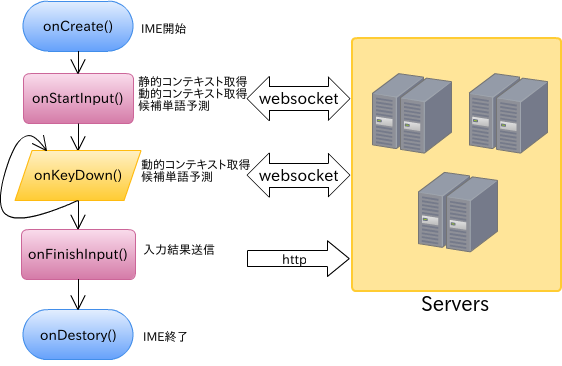
\includegraphics[width=14cm,bb=0 0 562 366]{images/clientflow}
  \end{center}
  \caption{Rive Clientフローイメージ}
  \label{fig:clientflow}
\end{figure}

\subsection{コンテキスト取得}

取得するコンテキストについては\ref{sec:getcontext}項を参照。
コンテキストはユーザーに入力してもらえるものは入力してもらう。
またデバイスで取得可能なものを全て取得し、推薦システムに使う。

\section{Rive Server}
\subsection{システム構成}

サーバーの中身は大きくRoutting Server,beforeRules,afterRules,Jubatusの
4つを実装した。
それぞれ候補単語の計算手法が異なるため此のような分割になっている。
\begin{figure}[htbp]
  \begin{center}
    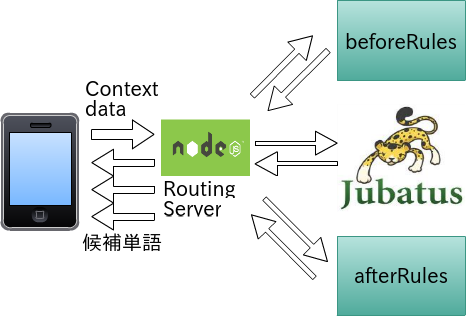
\includegraphics[width=14cm,bb=0 0 466 316]{images/riveserver.png}
  \end{center}
  \caption{Rive Server概要図}
  \label{fig:riveserver}
\end{figure}

\subsection{Routing Server}
このサーバーはふたとおりの役割を持っている。
一つはデバイスから受け取ったコンテキストデータを
beforeRules,Jubatus,afterRulesの3つの計算エンジンに振り分け送信する役割である。
もうひとつは受け取ったデータを受け取り次第、デバイスに送信する役割である。

\subsection{beforeRules}
このエンジンはコンテキストデータが送られてきた際に、
一定のルールに基づいているものをまとめている。
このルールは著者?開発者?がよく使われる単語を推測し実装した。
例えば、Twitter\cite{twitter}クライアントに入力を行っている(行おうとしている)
場合に「なう」「@」の候補単語を返すようになっている。

\subsection{Jubatus}
このエンジンについては第\ref{sec:jubatus}項参照。

\subsection{afterRules}
このエンジンはbeforeRulesより重要度が低く、
また計算に時間がかかるものを推測して実装した。
例えば、最寄り駅をクエリとしてその駅を通っている電車の線を
その場でWEBから検索し推薦単語として返すことができる。

\section{Rive Analytics}
このシステムはRive Client\ref{sec:riveclient}でのプロセスの終わりに
送られてくるデータを受信し、解析するシステムである。
開発者はこのシステムを使用することによって、新しい機能の有用性などを
確かめることができる。

\subsection{指標値}
\begin{itemize}
  \item CPI(click per input)
    入力がどれだけどうか
  \item CPI
  \item CPI
\end{itemize}

\section{Rive BatchProcessing}
このシステムは定期的に処理を行うものを管理し実行している。

\section{Rive WebService}
このシステムはインターネット上で閲覧可能なホームページである。
Riveシステムを試用することができる。


\chapter{評価実験}
\label{chap:application}

Rive日本語入力におけるシステムの有用性を検証する

\section{入力速度の向上}
\section{豊かな入力}

\chapter{議論}
\label{chap:discussion}

\section{処理単位としての人}

\chapter{関連研究}
\label{chap:related}
本章ではRive日本語入力に関連した研究について述べる。

\newpage
\section{IMEに関する研究・製品}
Rive日本語入力と既存の研究や製品を比較することで、
Rive日本語入力の特色を述べる。

\subsection{コンテキストアウェアIMEの実現へ向けた動的辞書生成手法の提案}
荒川らが研究・提案した動的辞書生成手法である。\cite{dynamicdictionarygeneration}
コンテキストを利用し、
様々な人のデータをひもづけることによって一つの辞書を作るという点に置いて
Rive日本語入力と類似している。
差異はコンテキストのリアルタイム性にある。
Rive日本語入力においてコンテキストは
動的コンテキストと静的コンテキスト\ref{recommmend}
に分かれているが、この動的辞書生成においては静的コンテキスト
として私が定義したものしか考えられていない。
またこのシステムではコンテキストについて位置情報についてのみ
考察しているがRive日本語入力では、
複数のコンテキストを総合的に解析する手法について設計し開発した。

\subsection{Social IME}
奥野が開発したユーザ間で辞書を共有するIMEである。\cite{socialime}
Rive日本語入力において複数のユーザが一つの辞書を利用するという
集合知を用いた辞書の発想は類似している。
このIMEにおいて使われているシステム\cite{奥野陽:2009-03-18}では
以前の入力などと言ったコンテキストが考慮されおらず、
Rive日本語入力ではそれらをコンテキストに導入することで、
文章全体における共起表現などの推薦を可能にした。

\subsection{iWnn}
omron社が開発した日本語IMEであり、\cite{iwnn}
現在AndroidOSにおいて多くの機種で標準搭載しているものである。
携帯電話向けに実装されていて、
時間情報やメールの送信相手の情報からコンテキストを推測し、
適切な推薦を行う点に置いて、Rive日本語入力と類似している。
コンテキストについては開発者の決めたものから推測するため、
未知のコンテキストなど柔軟なコンテキスト推測ができないところが、
Rive日本語入力システムと異なる。

\subsection{Google日本語入力}
Google日本語入力はGoogle社によって開発されたIMEである。
Googleの検索システムと連動しており最新かつ膨大な情報を使った
辞書が利用可能である。
検索システムを使っているため、
集合知を使いリアルタイムな情報を得たいという点に置いて
Rive日本語入力と類似している。
その上で実現するためのアプローチが異なっている。
Google日本語入力ではコンテキストとして利用されるものが過去の入力
だけになっている。

\subsection{各種クライアント}
Rive日本語入力システムにおいてコンテキスト推測で、
アクテビティー(第\ref{staticcontext})ごとに特化型クライントが存在する場合、
それらはIME機能を備えていることが多い。
Twitterクライアントであれば、
リプライを送る際に相手のアカウント名が自動で
入力されるようになる等の入力補助がある。

\section{コンテキストを使用した推薦システム}
コンテキストを利用したシステムに関する研究は始め、
位置情報や時間情報利用したシステムが多かった。
その後、そこにユーザー情報を加えたシステムの研究が行われた。
更にその後には、他のコンテキストを加えたシステムの研究が行われた。
\cite{okukenta}

\subsection{コンテキストの分類}
Rive日本語入力においては\ref{chap:recommend}において
述べたように実装上、動的コンテキストと静的コンテキストの
2種類に分類したが、
Strangらの研究\cite{contextsurvey}によると以下に分類される。
\begin{itemize}
  \item Key-Value Models
  \item Markup Schema Models
  \item Graphical Models
  \item Object Oriented Models
  \item Logic Based Models
  \item Ontology Based Models
\end{itemize}
しかしこの分類は結果を見すえた上での分類であり、
コンテキストがどのような推薦結果を提示するのか
予測が難しいRive日本語入力における
コンテキストの分類には適さなかった。

\subsection{}

\chapter{結論}
\label{chap:conclusion}

\section{おわりに}

\chapter{本研究に関する発表}
\label{chap:publications}

\section{学会}
\begin{itemize}
  \item 馬場匠見, 橋本翔, 増井俊之 実世界プログラミングのための分散人力処理環境,
        第6回データ工学と情報マネジメントに関するフォーラム 口頭発表
        [学生プレゼンテーション賞]
  \item 馬場匠見, 橋本翔, 増井俊之 Babascript: 人とコンピュータの協調による処理実行環境,
        第22回インタラクティブシステムとソフトウェアに関するワークショップ, 登壇発表
\end{itemize}

\section{展示会}
\begin{itemize}
  \item SFC OpenResearchForum2013 (2013年11月22日〜23日 東京ミッドタウンホール \& カンファレンス、主催:慶應義塾大学SFC研究所)
\end{itemize}

\section{その他}
\begin{itemize}
  \item 独立行政法人情報処理推進機構 2013年度未踏IT人材発掘・育成事業

        テーマ名: 実世界プログラミングのための分散人力処理環境の開発
\end{itemize}


\begin{acknowledgment}

このテンプレートを改造するにあたって、@kurokoboとインターネット上のいくつかの修士論文などを参考にしました。感謝いたします。

\end{acknowledgment}
  % 謝辞。要独自コマンド、include先参照のこと


\begin{bib}[100]
% BibTeXを使う場合
\bibliography{main}

%\begin{thebibliography}{#1}
%
%  \bibitem{参照用名称}
%    著者名:
%    \newblock 文献名,
%    \newblock 書誌情報,出版年.
%
% \bibitem{hoge09}
%  ほげ山太郎,ほげ山次郎:
%  \newblock ほげほげ理論のHCI分野への応用,
%  \newblock ほげほげ学会論文誌,Vol.31,No.3,pp.194-201,2009.
%
% \bibitem{hoge08}
%   Taro Hogeyama, Jiro Hogeyama:
%   \newblock The Theory of Hoge,
%   \newblock {\it The Proceedings of The Hoge Society}, 2008.
%
%end{thebibliography}

\end{bib}
  % 参考文献。要独自コマンド、include先参照のこと
\appendix
\chapter{付録の例}

付録を無理矢理出力させるため、てきとうなことを書く。

\section{ほげ}

コマンドは本文と一緒。

\subsection{ふー}

本文と一緒。

\section{ほげほげ}

本文と一緒。

\subsection{ふーふー}

本文と一緒。
    % 付録

\end{document}
